%%% template.tex
%%%
%%% This LaTeX source document can be used as the basis for your technical
%%% paper or abstract. Regardless of the length of your document, the commands
%%% are all the same.
%%% 
%%% The "\documentclass" command is the first command in your file. If you want to 
%%% prepare a version of your article with line numbers - a "review" version - 
%%% include the "review" parameter:
%%%    \documentclass[review]{acmsiggraph}
%%%

\documentclass{acmsiggraph}

%%% Title of your article or abstract.

\title{The Effect of Pop-Up Tutorials on Flow in Platformers}

\author{Calvin Brizzi\thanks{e-mail:calvin.brizzi@gmail.com}\\BRZCAL001}
\pdfauthor{Calvin Brizzi}

%%% Used by the ``review'' variation; the online ID will be printed on 
%%% every page of the content.

%\TOGonlineid{45678}

% User-generated keywords.

\keywords{flow, tutorials}

% With the "\setcopyright" command the appropriate rights management text will be added
% to your document.

\setcopyright{none}
%\setcopyright{acmcopyright}
%\setcopyright{acmlicensed}
%\setcopyright{rightsretained}
%\setcopyright{usgov}
%\setcopyright{usgovmixed}
%\setcopyright{cagov}
%\setcopyright{cagovmixed}
%\setcopyright{rightsretained}

% The year of publication in the "\copyrightyear" command.

\copyrightyear{2016}

%%% Conference information, from the completed rights management form.
%%% The "\conferenceinfo" command has two parameters: 
%%%    - conference name
%%%    - conference date and location
%%% The "\isbn" field includes the year and month after the article ISBN.

%\conferenceinfo{SIGGRAPH 2016 Posters}{July 24-28, 2016, Anaheim, CA} 
%\isbn{978-1-4503-ABCD-E/16/07} 
%\doi{http://doi.acm.org/10.1145/9999997.9999999}

\begin{document}

%%% This is the ``teaser'' command, which puts an figure, centered, below 
%%% the title and author information, and above the body of the content.

 %\teaser{
 %  \includegraphics[height=1.5in]{images/sampleteaser}
 %  \caption{Spring Training 2009, Peoria, AZ.}
 %}

\maketitle

\begin{abstract}

We present the results from an experiment (n=10) which uses a standard measure of flow to investigate the effect of pop-up tutorials on player experience.\\
The results, while not statistically significant, suggest that pop-up tutorials may have a positive effect on flow but require further studies.

\end{abstract}

%
% The code below should be generated by the tool at
% http://dl.acm.org/ccs.cfm
% Please copy and paste the code instead of the example below. 
%
\begin{CCSXML}
<ccs2012>
<concept>
<concept_id>10003120.10003121.10003122.10003334</concept_id>
<concept_desc>Human-centered computing~User studies</concept_desc>
<concept_significance>300</concept_significance>
</concept>
</ccs2012>
\end{CCSXML}

\ccsdesc[300]{Human-centered computing~User studies}

%
% End generated code
%

% The next three commands are required, and insert the user-generated keywords, 
% The CCS concepts list, and the rights management text.
% Please make sure there is a blank line between each of these three commands.

\keywordlist

\conceptlist

\printcopyright

\section{Introduction}
Csikszentmihalyi originally described flow as a mental state of being absorbed in activity while experiencing positive feelings \cite{optimal}. He also described a series of factors associated with flow, that were later refined specifically in the context of games by Chen [2007] to three core elements a game needs to evoke a flow experience:
\begin{itemize}
\item It is rewarding, and the player wants to play the game.
\item It offers a challenge that matches the player’s ability, allowing them to be absorbed into the game.
\item The player feels in control of the game activity.
\end{itemize}
Flow is an extremely desirable outcome for games and it incorporates a lot of the feelings that people associate with ``fun'' \cite{flow}.

Teaching new players how to play a game is a challenging but important part of game design. Tutorials are one of the main mediums game designers use to help players quickly acquire the necessary skills while still being within the play experience (opposed to say instruction manuals, where the player learns outside of the game). 
%%% THAT SUCKS, WRITE BETTER! ^^^^
When starting a new game the tutorial is, by design, the first experience players have. With some taking several hours to complete (Final Fantasy XIII being an extreme example where the players only get full control after thirty hours of gameplay), a poor first impression can often deter new players from returning to the game \cite{useMMO}. Furthermore, when research has been done on heuristics for evaluating fun in video games, providing ``an interesting and absorbing tutorial'' \cite{federoff} or similar phrasings \cite{desurvire} are frequently on the list, without any indication on what makes a tutorial ``absorbing''.

Recognizing what makes a good tutorial has benefits outside of games: the learning principles that are present in games are strongly supported by current cognitive science research and can be applied to learning in other contexts \cite{videolit}.\\
While the importance of tutorials is widely recognised, little research has been done on the effects of tutorials. The studies that are available are focused more around measuring time spent playing and return rate of players \cite{andersen}, or are conducted on such small test groups that any promising results do not achieve statistical significance \cite{hill}. 

The research on tutorials is particularly lacking when it comes to their relationship to flow. While many articles are available online about what makes a ``fun'' tutorial, none are backed by data. We believe a more rigorous analysis of tutorials would prove beneficial for the design of video games and other learning experiences.

As one of the main elements of flow is that of action-awareness merging \cite{jackson} we expect that any interruption to the action (such as the game stopping to give the player instructions) will ‘snap’ the player out of this state and require a certain amount of uninterrupted play to re-enter it.
On the other hand, optimal flow state is achieved when the challenge meets but does not exceed the player’s current skill \cite{nakamura}. We expect this specific game, due to it’s non-standard game mechanics (the player control two independent entities in the game, one per hand), to benefit greatly from a tutorial, accelerating skill acquisition \cite{andersen}. We also believe that a more obtrusive tutorial would be more effective at teaching the player.\\
We hope to discover how these two competing effects (the interruptions breaking the action, but increasing the skill level of the player) ultimately influence flow. After reviewing the many available measures of flow, we  identified the Short Flow State Scale (S FSS)\cite{jackson} as the one that most closely met our needs. It is a widely cited compact questionnaire (9 questions) that allows us to evaluate the flow state of each player on a scale of one to five.

The benefits of using Squishy Block as the underlying game are numerous. We were familiar with the source code which made rapid modification and iteration possible. It also fairs well in heuristic evaluations. For example, GameFlow identifies eight major heuristics for evaluating flow in games: concentration, challenge, control, player skill development, clear goals, feedback, immersion and social interaction \cite{sweetser}. The non-standard game mechanics requires concentration to use and is a challenge even for experienced players but, once the skills are developed, give a feeling of control within the game. Like all platformers, there is always a clear, achievable goal (to reach the end of the level) and feedback on progress is given at the end of each level. Finally, the combination of all the above elements, along with upbeat music, makes it a game that is easy to get immersed in \cite{sanders}. Social interactions is the only heuristic that it fails to perform in, but introducing a multiplayer element could introduce too many confounding variables.\\
While heuristic evaluations do have limited usefulness, they are still helpful in identifying issues before players interact with the system \cite{desurvire}, reducing further the risk of something other than our modifications having an effect on the flow score. 

This paper details an experiment designed to investigate the effect a pop-up tutorial has on flow and the results collected from 10 subjects who participated.  
By collecting information on the speed at which each player complete post-tutorial levels, we also hope to achieve a better understanding of the effect the pop-up tutorial has on the speed at which the players acquire the skills needed to play the game.

Particular attention was also given to players' self-rated previous experience with platformers. We suspected this could be a major confounding factor when it came to players' S FSS score and the speed at which they completed the tutorial-free level.

\section{Experiment}

We conducted this experiment as part of the User Experience in Games module of the Computer Science Honours Degree at the University of Cape Town. Two separate groups of users each playing a slightly different version of the same game were used. One group acted as a control and played a version where the tutorial prompts were part of the game's background, incorporated into the level. The other group played a version of the game where at specific intervals a pop-up screen would interrupt the game with instructions for the player. The flow scored collected across the two groups were compared.\\
The purpose of the experiment was to investigate the effect the pop-up tutorial would have on flow while simultaneously timing players on a second, tutorial free level to measure the effect the different versions of the game would have on skill acquisition speed.

\subsection{Participants}

We recruited 10 unpaid volunteers from the second and third year computer science courses. We did not collect demographic information. Participants were initially randomly assigned to one of the two conditions until the final participants who were assigned to maintain an even number of players for each version.\\
Before beginning they each confirmed that they'd never played the game before (as a version is freely available online)\cite{ssbb}, had not participated in any other User Experience in Games experiments and provided consent for the data to be collected.

\subsection{Game}

The game used was Squishy Block, a simple 2D platformer. The game has many of the standard platformer mechanics (the character can move and jump, enemies damage player on touch, power-ups are located at various points in the level, progression is from left to right) while adding a novel element in the form of an independently controllable block that the player must use to help their character overcome obstacles that the player cannot simply jump. The block also provides the only way for the player to kill the enemies present in each level, as they will otherwise pursue the player until they make contact, damaging the player. \\
The game was modified to have two versions: a background tutorial version and a pop-up tutorial version.
In the background version, shown in Figure \ref{fig:even}, information on how to play was displayed on small scrolls that were incorporated into the level (close-up shown in Figure \ref{fig:close}). The user could not interact with the signs in any way and they had no effect on gameplay. They were placed at fixed positions throughout the level.\\
 \begin{figure}[!b]
  \centering
  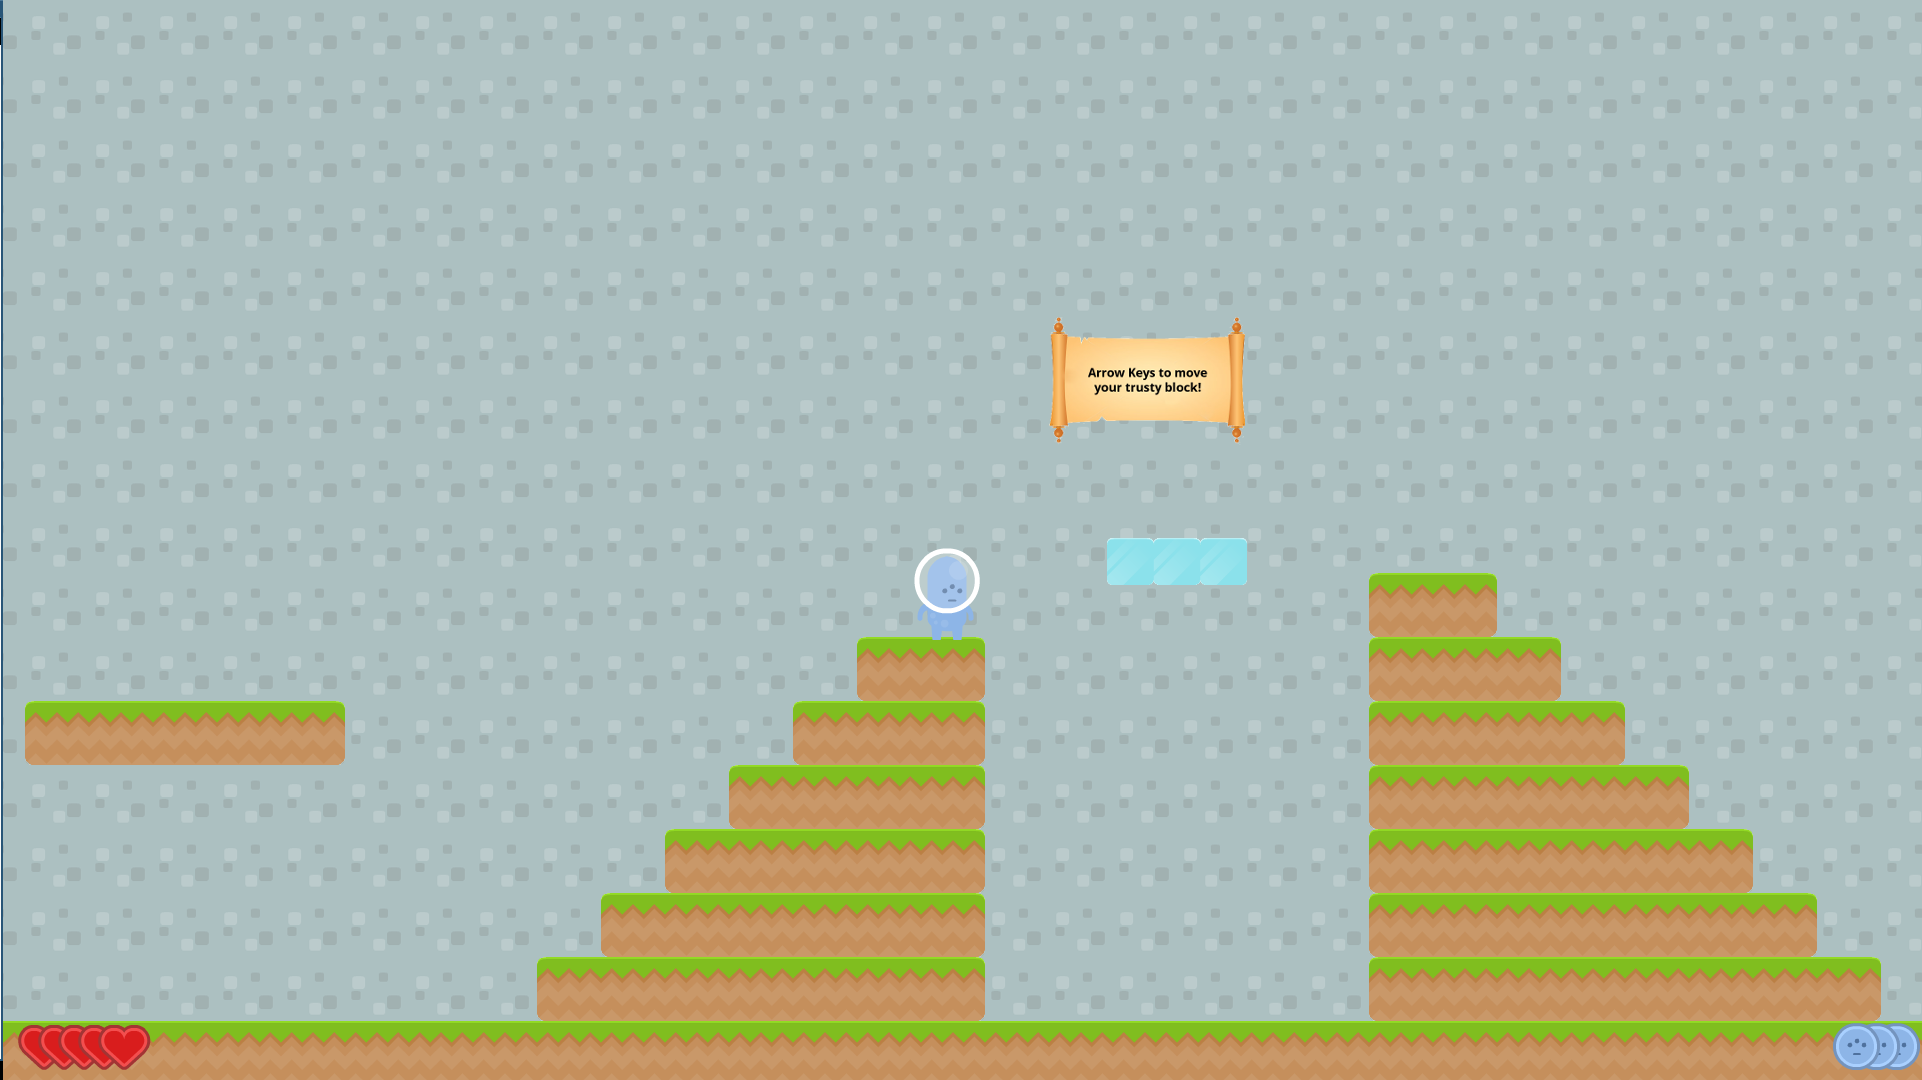
\includegraphics[width=3.0in]{images/even}
  \caption{The background version of the tutorial}
  \label{fig:even}
\end{figure}
\begin{figure}[!h]
  \centering
  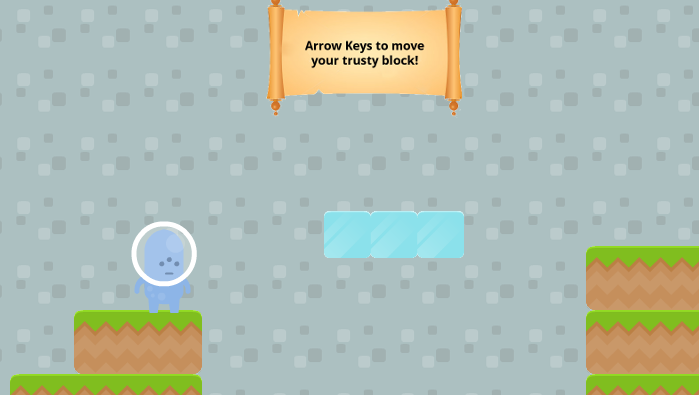
\includegraphics[width=3.0in]{images/close}
  \caption{Close-up of the background version}
  \label{fig:close}
\end{figure}

\begin{figure}[!h]
  \centering
  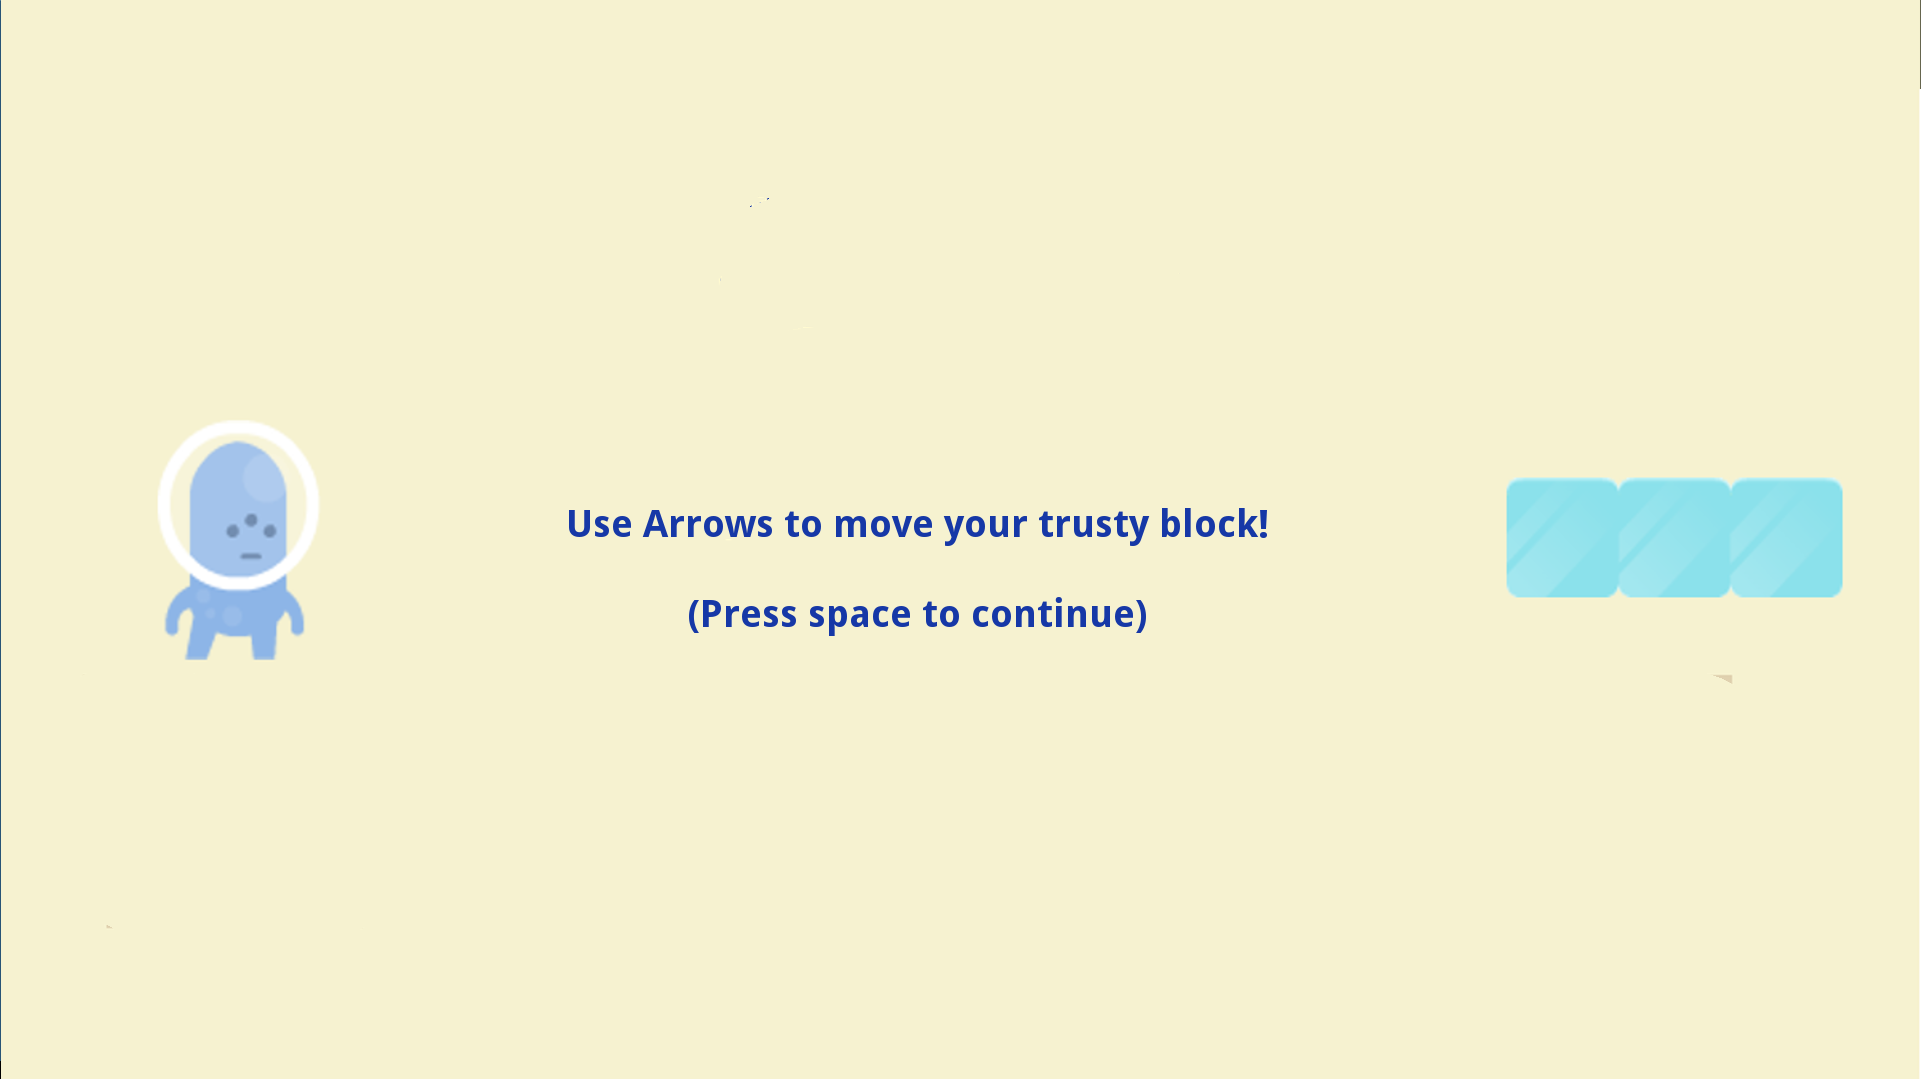
\includegraphics[width=3.0in]{images/odd}
  \caption{The pop-up version of the tutorial}
  \label{fig:odd}
\end{figure}
In the pop-up version, shown in Figure \ref{fig:odd}, information on how to play was displayed in full-screen pop-ups that needed to be manually dismissed by the player before the game could be resumed. Both versions had five points at which information was displayed. 

It is important to note that the game was identical in every other way. The text displayed in the pop-up and background prompts was the same and the pop-up prompts triggered at the same point that the background signs were visible in order to ensure any differences in experience were as a result of the format of the tutorial and not the contents. The different versions also had an identical soundtrack and sound effects.

The game was modified to have two levels; the first contained the tutorial which introduced the player to the controls and concepts of the game gradually, as those controls or concepts became necessary (for example explaining how to deal with enemies just before the first enemy was encountered). The second level had no tutorial elements and was designed to test the player on everything introduced in the first level. The players were unknowingly timed on the second level.


\subsection{Location and Equipment}
The experiment was conducted in an isolated room, with only the experimenter and the subject present to reduce possible distractions.
The subject was also given a pair of noise-isolating headphones that were worn while playing the game but removed otherwise.
All subjects used the same machine to fill out questionnaires and play the game: a laptop with an Intel i7 processor and integrated Intel HD 5500 Graphics. The game is lightweight and therefore ran at a stable 60fps on the laptop's built-in display which has a resolution of 1920x1080.\\
All subjects used the same generic external keyboard during play and a generic USB mouse was provided but only used while filling out the forms (the game controls are entirely keyboard based). \\
Questionnaires were filled out in the Chrome browser using Google Forms and data was later analysed using Excel's built-in data analysis features.

\subsection{Procedure}
The experiment was conducted in three phases: an initial brief questionnaire, the game itself and then a final questionnaire.\\
In the initial phase subjects were briefed on how the experiment would be conducted, gave their consent to participate in the study and were asked to rate their previous experience with platformers. They then switched over to the game and played through the two levels (or until their character died three times) before completing the final questionnaire: the Short Flow State Scale (S FSS)\cite{jackson}. Finally, the experimenter filled in data about what version of the game the participant had played and the time taken.
The players were given no instructions on how to play the game before launching the game (as this was guided by the tutorial). The entire process took less than 10 minutes, depending on how quickly players completed the two levels.\\
Participants were then debriefed: all the data being collected was explained to them, the objective of the study was made clear and they were encouraged to ask questions if they had any.

\section{Results}
The S FSS is a series of 9 questions, which a player then answers on a 5 point Likert scale. The responses are then averaged for each player to get their flow score.

Descriptive statistics for the samples are shown in table \ref{SFSS descriptive} and table \ref{time}. Some subjects did not complete the second level, which was not expected, so their time results were not included. This unfortunately further reduced the already small sample size.

The S FSS score and time data was analysed using a two-tailed unpaired t-tests to test for differences in the means of the flow score between the two versions. The results are presented in table \ref{ttest}.
In an attempt to determine whether or not it was a confounding variable we also analysed the correlation between player experience in game and the above variables. The results are presented in table \ref{corr}.
\\


\begin{table}[h]
  \centering
  \caption{S FSS Score descriptive statistics}
  \label{SFSS descriptive}
  \begin{tabular}{|c|c|c|c|}
  	\hline
  	\textbf{Version} & \textbf{Mean} & \textbf{Standard Deviation} & \textbf{N}\\
    \hline
    background & 3.62 & 0.45 & 5 \\
	pop-up & 4.02 & 0.51 & 5 \\
    \hline
  \end{tabular}
\end{table}

\begin{table}[h]
  \centering
  \caption{Completion time descriptive statistics}
  \label{time}
  \begin{tabular}{|c|c|c|c|}
  	\hline
  	\textbf{Version} & \textbf{Mean (s)} & \textbf{Standard Deviation (s)} & \textbf{N}\\
    \hline
    background & 115.25 & 29.33 & 4 \\
	pop-up & 85.67 & 9.29 & 3 \\
    \hline
  \end{tabular}
\end{table}

\begin{table}[h]
  \centering
  \caption{Unpaired t test result}
  \label{ttest}
  \begin{tabular}{|c|c|c|c|}
  	\hline
  	\textbf{Dependent variable} &\textbf{t}  &\textbf{p} & \textbf{Difference of means}\\
    \hline
    S FSS Score & 1.3235 & .2223 & 0.40 \\
    Time & 1.6506 & .1597 & 29.58\\
    \hline
  \end{tabular}
\end{table}

\begin{table}[!h]
  \centering
  \caption{Analysis of correlation with previous experience}
  \label{corr}
  \begin{tabular}{|c|c|c|}
  	\hline
  	\textbf{Variable} &\textbf{r} & \textbf{p}\\
    \hline
    S FSS Score & 0.7953 & .0030 \\
    Time & -0.8749 & .0060\\
    \hline
  \end{tabular}
\end{table}

\subsection{Discussion}
With a two tailed unpaired t-test we found no significant effect on S FSS Score (t(10)= 1.3235, p\textgreater  0.05) or time to complete (t(7)=1.6506, p\textgreater0.05). We however did find that previous experience is strongly correlated to both S FSS Score (r(10)= 0.79, p\textless0.01) and time to complete (r(7)=-0.87, p\textless0.01).

As we can see, not only are the results of the t-test statistically insignificant, likely influenced by the small sample size, but player's previous experience is a major confounding variable. Due to the small sample size, there is no statistically sound way to control for this, making the results for the unpaired t-test less useful.
 
So while the results seem to imply that pop-up tutorials, even though they interrupt the game initially, create an increase in scores on the S FSS, the means are comfortably within one standard deviation of one another and any difference may be explained by the fact that the pop-up version of the game included participants who generally rated their previous experience with platformers higher than the participants who played the version with a background tutorial. 

\section{Conclusion and Future Work}
Unfortunately, the only real conclusion that can be reached from the results is that players with more experience in platformers enjoy platformers more and are much quicker at beating them. Neither of these results are particularly surprising nor relevant when it comes to examining the effects of different tutorial formats on flow or player learning speed.

There are various criticisms that can be directed at this experiment. Most importantly, the sample size is too small to be able to reach statistically significant conclusions. Secondly, the game selected, while simple in concept, can be frustratingly hard for low-experience players and subsequent research should consider selecting only participants who are already comfortable with platformers. Finally, senior Computer Science students may not be representative of the gaming population, and alternative recruitment strategies might be necessary.

A repeat of this experiment, with more participants selected based on their previous experience in platformers would give better insights into what format a tutorial should have while also allowing alternative tutorial formats to be evaluated (for example audio instructions).

Further research in this area could be beneficial in enabling game creators to design tutorials in a way that aids flow in the game, creating an overall better experience for players and retaining them for longer. The benefits to other disciplines like education should also be considered. Serious games for example, can be seen as extended tutorials designed to educate the player while still keeping them engaged in the game itself.

\section*{Acknowledgements}

Prof Edwin Blake and Jacob Clarkson for feedback on experiment proposal and design.

\bibliographystyle{acmsiggraph}
\nocite{*}
\bibliography{brzcal001-UXG-Exam}
\end{document}
